
\section{Proposal}
\label{sec:prop}
% Proposal:
%  - retomar problema {iot, sec, ND};
%  - objetivo;
%  - soluções {minas, paralelismo, distribuído, ~~py-kafka, flink,~~ mpi}
%  - propor uma solução

% \begin{highlight}
% A expansão do IoT na industria e vida diária\\
% leva a maior incidência de intrusão e subversão\\
% portanto são necessários sistemas de detectão de intrusão\\
% eficases (boa acuracia) e eficientes (baixa latência)\\
% portanto propôen-se\\
% um NIDS que utiliza algoritmo de detecção de novidades (para acurárcia)\\
% implementado de maneira distruída na borda e nuvem (para latência).\\
% \end{highlight}

Amid of \iot expansion in multiple fields, from industry to daily life,
the constant threat of intrusion
% , subversion (overthrow), denial of service
(or any other unexpected detrimental behavior)
% by any component of a system or external actors
is a prospect looming over many systems administrators
and for that reason
% Thus, 
new network surveillance tools are needed, especially 
effective (accurate) and efficient (fast reaction and good throughput) \nids.
% Following that reasoning, new \nids and other autonomous and analytic system
% surveillance tools are being proposed, many employing techniques such as Anomaly
% and Novelty Detection.
% These tools require the network packet traffic to be constantly analysed,
Thus we propose a \nids using MINAS \cite{Faria2016minas} (a Novelty Detection algorithm)
to effectively identify previous and new intrusion threats,
implemented over a architecture \cite{Cassales2019a} using parallel and distributed techniques leveraging
edge and cloud for efficient computing.

\hl{[start] intro/related?}

\nids 
monitor the packet network traffic, aggregate into flow descriptors and
% aggregated into flow descriptors and further processed in a classification
analyze to identify any intrusion or misbehavior.
% using methods such as classification and Novelty Detection
% This requirement in turn, requesting more computing power at the edge.
% While requesting more computing power in a cloud environment is trivial and
% inexpensive, the same cannot be said 
However, this problem requires both fast and accurate response:
the former is needed to have a proper reaction before harm can be cast
to the network and to cope with the traffic without imposing loss or delay
in the \nids or observed network;
the latter is required as to not misidentify harmless with harmful and vice-versa.
To achieve those goals we leverage fog computing.

% \hl{intro/related?}

In common \iot scenarios, data is captured by small devices and sent to the
cloud for any compute or storage tasks, however this is not feasible in our
\nids scenario, even though we also capture data produced in the edge,
sending this data to the cloud would in the worst case double the
internet communication requirements of the overall system.
Fog computing infrastructure aims to offload
computing resources from cloud providers by placing edge
devices closer to end-users and/or data sources.
But two MINAS steps limit this fog offload,
the processing intensive novelty detection and,
long term model storage and distribution of the internal model.
Those steps surpass the capabilities of common fog hardware and
therefore need to be at least shared to a cloud where such
requirements are easy and cheap to fulfill.

\hl{[end] intro/related?}

In our proposed \nids, fog and cloud computing resources are
employed as to minimize the time elapsed between a flow descriptor
ingestion and intrusion alarm, allocating the 
classification step of MINAS in a MPI cluster running multiple
classifier instances.
After the initial classification, the resulting label can be used immediately,
but if the sample is labeled as \emph{unknown}, this sample must be stored
and the novelty detection step will be triggered, and those steps require more resources
and thus are divided in fog and cloud.

% Therefore, our objective is a Distributed novelty detection in streams using limited hardware.
% Previous attempts to attain the objective of distributed fast

\begin{figure}[b!]
  \centerline{
    \begin{subfigure}{.5\textwidth}
      \centering
      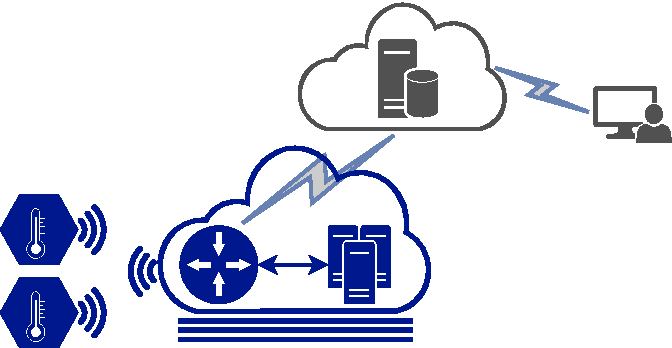
\includegraphics[width=0.9\linewidth,page=1]{figures/mfog-arch-fisica.svg.pdf}
      \caption{\mfog physical architecture overview with cloud model storage.}
      \label{fig:mfog-phy-arch-cloud}
    \end{subfigure}
    \begin{subfigure}{.5\textwidth}
      \centerline{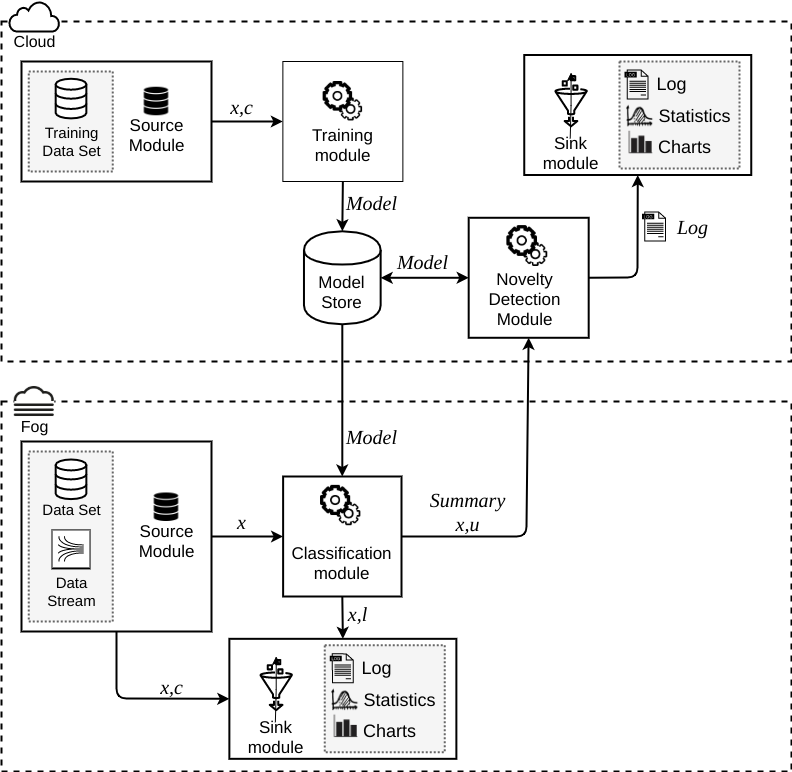
\includegraphics[width=0.9\linewidth]{figures/mfog-arch-v2_en.png}}
      \caption{\mfog components and communications overview.}
      \label{fig:mfog-architecture}
    \end{subfigure}
  }
  \caption{Architecture overview.}
  \label{fig:arch-overview}
\end{figure}

The overall organization of components, connections and interactions with external
actors is shown in Figure \ref{fig:mfog-phy-arch-cloud},
from bottom left to top right: sensor network; fog containing gateway router
and novelty detection cluster; cloud storage for model, alarms and statistics
and; human supervisor addressing alarms and statistics.

In Figure \ref{fig:mfog-architecture} we depict each logical component associated
with each MINAS step and its communications, we also depict extra modules for sampling
and measurements.
Each communication in Figure \ref{fig:mfog-architecture} shows the direction of the data flow
and identifies the data contained:
$Model$ is MINAS internal Model containing a set of cluster data structures,
$x,c$ identifies a sample with the real class,
$x$ is the sample without the real class,
$x,l$ identifies a sample with the assigned label,
$x,u$ is  sample with the \emph{unknown} label,
$summary$ is a statistical summary of model usage.

\subsection{Polices}\label{sec:polices}

The distribution of steps and tasks in various modules opens
data distribution and its impacts to discussion.
The decisions following these discussions can be organized in
several policies, some of them are:

\begin{itemize}
    \item Regarding the allocation of the Novelty Detection Module:
    \begin{itemize}
        \item 
        It can be located at each fog node meaning novelties will be only
        detected if sufficient patterns occurs in the local observed network,
        it also spends the local node processing power and a model sharing mechanism 
        must be added;
        \item It can be located in the cloud and thus detect patters even when
        their footprint is small in each local network, also a model sharing mechanism
        is not needed as the model has a single instance stored in the cloud,
        the penalty of this choice is increased internet usage as any sample with
        \emph{unknown} label must be sent from edge to cloud, implying some delay
        between the appearance of a novel pattern, its detection and its propagation
        to fog classifiers;
        \item It can be located in both, meaning that a local \emph{unknown} buffer
        is maintained, novelty detection is performed on that buffer, and once
        a sample is to be discarded as noise or outlier it must be sent to the cloud
        where the process repeats but with global data. This choice also need the model
        sharing mechanism and is clearly the more complex.
    \end{itemize}
    \item Regarding the model cleanup (forget mechanism):
    Even when a global novelty detection is used, local models can be optimized for faster
    classification using the its local model statistics, sorting last or removing clusters that
    are not in frequent use;
    \item Lastly, a feature not explicitly shown in the original MINAS is the reclassification
    of \emph{unknowns} after the detection of a novelty pattern with the newfound label:
    As the last step in the novelty detection step in MINAS, the \emph{unknown} sample buffer is
    classified using the newfound subset of clusters, if the sample can be explained by a new cluster
    it is removed from the \emph{unknown} sample buffer, however, this new labeling is not put forward
    to the systems output restraining the system data-stream behavior to a \emph{map} (meaning each input
    has one output), whereas if this feature was enabled the behavior would be a \emph{flatMap} (each input
    can have many outputs) and introduce new outputs, more recent and perhaps more accurate but later.
\end{itemize}

% \begin{highlight}
% - Detecção de novidades e manutenção de modelo em ambiente distribuído:

%   - Mecanismo de ND local (síncrono) vs nuvem quanto à atraso de definição de modelo
%     (nesse ponto é onde a hipótese prevê maior diferença, grande ponto de interesse);

%   - Mecanismo de esquecimento local vs global (modelo único ou por nó);

%   - Atraso na reclassificação dos desconhecidos;
% \end{highlight}

\subsection{Implementation}\label{sec:implementation}

The original MINAS algorithm has a companion implementation (\refminas)
written in Java using MOA library base algorithms such as K-means and CluStream,
however in the new implementation only K-means is used.
% \refminas employs Java's double, a $64 bits$ number whose precision is not
% absolutely necessary and, as it is often necessary to shuffle between nodes via
% network and a small economy could be made with only a float number with $32 bits$.
Another difference between \refminas and \mfog is cluster radius calculation
from the distances of elements forming the cluster and the cluster's center,
where the former uses the maximum distance, the latter uses the standard deviation
of all distances as described in \cite{Faria2016minas}.

% Desafios de implementação:
% <!--
% - Definição de raio: desvio padrão das distâncias versus distancia máxima;
% - Atualização do micro-cluster limita-se à atualização do atributo \texttt{T};
% - Remoção de exemplos na implementação de referência é feita somente para o algoritmo \textit{CluStream};
% - Inclusão de borda: algoritmo inclui ($<=$), referência não inclui ($<$);
% - Seguiu-se as mesmas divergências anteriores para comparação dos resultados com a implementação referência;
% - Inclusão da borda;
% - Comportamento do mecânismo de \textit{sleep-model} não está definido, portanto não está ativo;
% - Processo de clusterização é limitado ao algoritmo \textit{K-Means}. Algoritmo \textit{CluStream} não está implementado;
% - -->
% - `Double vs Float`:
%   - Na implementação de referência, java double é utilizado;
%   - Na nova implementação duas versões foram testadas e a diferença de precisão entre as duas é de `5 E-8`;
%   - **Solução:** Use `float32` e economize os bits já que haverá comunicação entre nós e módulos;
% - Formato do fluxo de saída:
%   - Implementação de referência utiliza a tripla `(id, classe, etiqueta)`;
%   - Primeira implementação em C utiliza `(id, clusterLabel, clusterId, clusterRadius, label, distance, secondDistance)`;
%   - Segunda implementação utiliza dupla `(id, label)`;
%   - Na etapa de avaliação, independente de versão, o fluxo original é lido;
%   - **Solução:** O formato mínimo é `(id, label)`;

The stream format for input and output also of note.
Input information needed is the value of the item, this value is a number
sequence of length $d$ (referenced as dimension).
In addition to the value for evaluation and training purposes the class
identifier as single character, optionally an unique item identifier
(\textit{uid}) can be provided.
For output information and format the decision isn't so clear as we can't
predict future system integrations needs like only novelty alarms or every
item's original value with assigned label so, we have a compromise and put only
enough information for the Evaluation Module (where the full information
from the testing file or stream can be accessed) meaning the format can be
defined as a tuple containing \textit{uid} and assigned label.

% - Reprocessamento dos exemplos utilizados para atualização do modelo:
%   - Muda o comportamento do operador de fluxo de `Map` para `Flatmap`, ou seja,
%     requer outro fluxo de saída para a transmissão de padrões novidade (alarmes);
%   - Para reclassificação a definição de raio é modificada de `r = f * σ` (fator
%     multiplicando desvio padrão) para `r = max(distance)` (distância máxima);
%   - Passível da crítica de *overfitting*. Isto é, este processo pode
%     inflar a métrica de precisão;
%   - **Solução:** *em aberto*;

Another implementation decision related to the output stream is whether or not
to reprocess, and add to the output stream, examples in the unknown buffer after
the novelty detection procedure, meaning one item can be classified once as
unknown and again with a label.
Our preliminary tests using this technique had increased true positives when compared to
not using it.
However this changes the stream operator behavior from a \textit{Map} to a
\textit{FlatMap} having duplicate entries on the output stream as previously
mentioned.
Regardless of choice the classification of the unknown buffer after a model
update, using the full model or just the added set of clusters, is done to
remove the examples ``consumed'' in the creation of a new cluster in the internals
of the clustering algorithm.
% This removal can be made less complex if using only new clusters 

% Próximos desafios:
% - Distribuição e paralelização para minimização de latência entre novo item no fluxo e sua classificação:
%   - Tempo de passagem da instância pelo classificador;
%   - Volume máximo do sistema;
%   - Diferenças de precisão de acordo com a carga;

For \mfog the Message Passing Interface (MPI) library was used.
In MPI programming, multiple processes of the same program are created by the
runtime and each process instance receives a rank parameter, for \mfog this
parameters indicate if the process is root, rank $0$, or leaf otherwise.
Beyond this division, each process also operates two threads, for the root
there is a sampler and detector threads, for the leafs each has a model receiver
thread and multiple classifier threads.
The overall sequence of interactions is shown in \ref{fig:mfog-mpi-life}.

\begin{figure}[htb]
  \centerline{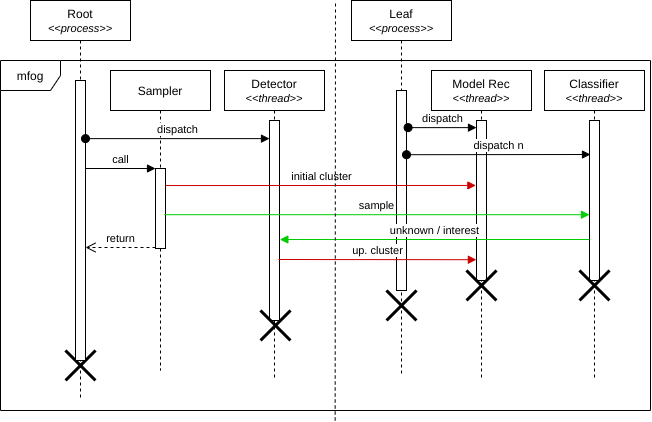
\includegraphics[width=0.5\textwidth]{figures/mfog-arch-mpi.png}}
  \caption{\mfog life line overview.}
  \label{fig:mfog-mpi-life}
\end{figure}

The Evaluation Module was also build following reference techniques like
multi-class confusion matrix with label-class association
\cite{Faria2016minas}
to extract classification quality metrics.
